\documentclass[11pt]{scrartcl}
\usepackage[utf8]{inputenc}
\usepackage{mathtools}
\usepackage{amssymb}

\usepackage{caption}
\usepackage{color}
\usepackage{xcolor}
\usepackage{listings}
\DeclareCaptionFont{white}{\color{white}}
\DeclareCaptionFormat{listing}{\colorbox{gray}{\parbox{\textwidth}{#1#2#3}}}
\captionsetup[lstlisting]{format=listing,labelfont=white,textfont=white}

\usepackage{tikz}
\usetikzlibrary{automata,positioning}


\title{\textbf{1810 Einsendeaufgabe KE 02}}
\author{Gustavo Nunes Martins}

\begin{document}
	\maketitle
	\section*{Aufgabe 1}
	Dieses Grammatik ist durch die B-Symbol links-rekursiv und nicht für rekursiven Abstieg geeinigt (unendliche loop). Man kann die links-Rekursion durch eine rechts-Rekursion ersetzen:
	
	\begin{center}
	$B \rightarrow yzzBV \mid AwV$
	
	$B' \rightarrow wzV \mid \varepsilon$
	\end{center}
	Die folgenden Syntax-Diagramme helfen, die Parser zu erzeugen. Die entsprechende Implementation ist nebenan:
	\subsection*{S:}
	\begin{minipage}{.5\textwidth}
	
\includegraphics[width=.3\linewidth]{../../../../Desktop/diagram/diagram/S}
	\end{minipage}
	\begin{minipage}{0.6\textwidth}
		\begin{lstlisting}[language=C]		
void CheckS(){
  CheckA();
}
		\end{lstlisting}
	\end{minipage}
	\subsection*{A:}
	\begin{minipage}{0.5\textwidth}
		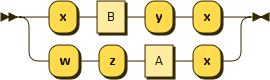
\includegraphics[width=1\linewidth]{../../../../Desktop/diagram/diagram/A}
	\end{minipage}
	\begin{minipage}{0.6\textwidth}
		\begin{lstlisting}[language=C]		
bool CheckA(){
  if (getchar()=='x') then 
    {CheckB();checkT('y');checkT('x');return TRUE}
  else if (getchar()=='w') then 
    {checkT('z');checkA();checkT('x');return TRUE}
  else error('A');
}
		\end{lstlisting}
	\end{minipage}	
	\subsection*{B:}
	\begin{minipage}{0.5\textwidth}
		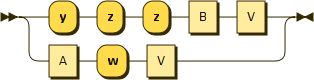
\includegraphics[width=1\linewidth]{../../../../Desktop/diagram/diagram/B}
	\end{minipage}
	\begin{minipage}{0.6\textwidth}
		\begin{lstlisting}[language=C]		
void CheckB(){
if (getchar()=='y') then 
  {checkT('z');checkT('z');checkB();checkV();}
else if (checkA()) then 
  {checkT('w');checkV();}
else error('B');
}
\end{lstlisting}
	\end{minipage}
	\subsection*{V:}
	\begin{minipage}{0.5\textwidth}
		
\includegraphics[width=.75\linewidth]{../../../../Desktop/diagram/diagram/V}
	\end{minipage}
	\begin{minipage}{0.6\textwidth}
		\begin{lstlisting}[language=C]		
void CheckV(){
  if (getchar()==' ') then 
    {}
  else if (getchar()=='w') then 
    {checkT('z');checkV();}
  else error('V');
}
		\end{lstlisting}
	\end{minipage}
\begin{lstlisting}[language=C]

int main(){
  checkS();
}
		
void CheckT(char terminal){
  if (getchar()!=terminal) then error(terminal);
}

void error(char location){
  printf("ERROR: Symbol %s failed\n", location);
  exit(-1);
}

\end{lstlisting}
	\section*{Aufgabe 2}
	\subsection*{a}
	Nur 2 Produktionsregeln sind verändert, nämlich:

	\begin{tabular}{l|l}
		vorher & naher \\ \hline
		$S \rightarrow aTbUcU \mid aTbU$ & 
		$S \rightarrow aTbUS', S'\rightarrow cU\mid \varepsilon$
		\\
		$T\rightarrow dVd \mid dVdW \mid dVdX$ & $T\rightarrow dVdT', T'\rightarrow \varepsilon\mid W \mid X$
	\end{tabular}
	\subsection*{b}
	\begin{tabular}{l|l|l|l}
		Regel & FIRST & FOLLOW & Steuer \\ \hline
		S & \{a\} & \{\$\} & \{\} \\
		S' & $\{\varepsilon,c\}$ & \{\$\} & \{\} \\
		T & \{d\} & \{b\}  & \{\} \\
		T' & $\{\varepsilon,e,f\}$ & \{b\}  & \{\} \\
		W & \{e\} & \{b\} & \\
		X & \{f\} & \{b\} & \\
		U & $\{h, g, \varepsilon\}$ & \{\$,c\} & \\
		Y & \{h\} & \{b\} & \\
		V & \{d\} & \{d\} & \\
		Z & $\{g,\varepsilon\}$ & \{\$,c,b\} &
	\end{tabular}
	\subsection*{c}
	TODO
	\section*{Aufgabe 3}
\end{document}